% !TeX spellcheck = nl_NL
%second chapter of your thesis
\chapter{Literatuurstudie} \label{ch:literatuurstudie}

In dit hoofdstuk zal er eerst een afgrenzing gegeven worden waarbinnen de thesis gekozen is. Vervolgens zal een korte introductie gegeven worden tot Artifici\"ele Intelligentie en Machine Learning waarin verschillende vormen en mogelijke toepassingsdomeinen behandeld worden. De verschillende leermodellen worden bekeken en er wordt nagegaan hoe de onderdelen een werkend geheel vormen. Vervolgens wordt er een overzicht van de voor- en nadelen van de verschillende technieken gegeven. Er wordt een best bruikbare methode voor de toepassing in deze thesis gekozen. Bij deze keuze zullen de voor- en nadelen gewikt en gewogen worden. Verder wordt er ook de geschiedenis van Single Board Computers aangehaald. Hoe zijn deze toestellen ontstaan, hoe zijn ze ge\"evolueerd en in welke staat zijn de hedendaagse SBCs. Verder worden ook verschillende voorbeelden van SBCs besproken die in staat zijn om Machine Learning-technieken toe te passen. Deze zullen onderworpen worden aan een benchmark die in paragraaf ~\ref{benchmark} besproken zal worden.


\newpage

\section{Kadering}

Een branche in de \gls{ml} die steeds meer in de schijnwerpers staat, is de logistieke sector\cite{barreto2017industry}. Door de steeds verder doorgedreven automatisatie van bedrijven, wordt er ook in bijvoorbeeld magazijnen geopteerd voor het optimaliseren van onder meer het leveren van de verschillende onderdelen en de veiligheid in het magazijn. Gebruik maken van zelfrijdende vorkheftrucks is een mogelijke optie in het verbeteren van de effici\"entie. Niet alleen in het magazijn maar ook op de weg is er een groeiende belangstelling naar zelfrijdende voertuigen, die ontwikkeld worden door grote bedrijven zoals Tesla en Uber. In beide cases zal er een zekere vorm van positiebepaling nodig zijn. Het is van groot belang dat deze bepaling zo accuraat mogelijk plaats vindt, met niet alleen een juiste locatie, maar ook een resultaat dat op zo kort mogelijke tijdsperiode geproduceerd wordt. 

Deze nood aan \textit{low latency} kan het verschil betekenen tussen een voertuig dat beslist dat hij moet vertragen of beslist dat hij veilig kan doorrijden maar toch een botsing veroorzaakt. De berekening van die cruciale locatiebepaling kan zowel in de \textit{cloud}, als in de \textit{edge}\cite{edgecomputingLi} gebeuren en gebeurt onder meer met behulp van \gls{ml}. Hierbij wordt met cloud verwezen naar het verwerken van data op een locatie ver weg van het voertuig zoals serverzalen. Met edge wordt dan weer een locatie dichtbij het voertuig bedoeld. Dit kan zowel op, als vlakbij het voertuig zijn. \textit{Cloud computing} brengt een zekere toegevoegde latency teweeg. Dit is de nodige tijd om via het internet de server te bereiken. Hierdoor zal men eerder kiezen voor \textit{edge computing} vallen. Indien de berekeningen in de edge plaats vinden zal er bijvoorbeeld een kleinere vertraging zijn tussen het moment van vertrekken en het waarnemen door het algoritme dat er vertrokken werd. De afstand tussen de re\"ele locatie, waar het voertuig zich fysisch ook bevindt, en de virtuele locatie, waar de computer het voertuig acht te zijn, is kleiner bij lagere latencies. Dit leidt tot een betere positiebepaling. Deze heeft dan weer tot gevolg dat meer ongevallen vermeden kunnen worden. Welke hardware men gebruikt kan vari\"eren van applicatie tot applicatie. De berekening zelf wordt uitgevoerd met behulp van \gls{ai} doordat dit verschillende baten heeft. Deze voordelen worden besproken in de volgende paragrafen.



\newpage

\section{Artifici\"ele Intelligentie}
\gls{ai} verwijst naar het simuleren van menselijk intellect in machines die geprogrammeerd worden om de menselijke redenering na te bootsen. Het wordt gezien als de studie van \textit{intelligente agents} die zijn omgeving waarnemen en acties kunnen ondernemen om de kans van het bereiken van een bepaald doel te maximaliseren\cite{poole1998computational}. Er kan een onderscheid gemaakt worden tussen zowel sterke als zwakke \gls{ai}.
\begin{itemize}
	\item \textbf{Zwakke \gls{ai}:} Dit is een vorm van \gls{ai} die zich bezig houdt met onderzoek in gebieden waar handelswijzen mogelijk zijn die tekenen van intelligentie vertonen, maar niet volwaardig intelligent zijn. Hier worden de meeste vorderingen in voortgebracht, zoals handschriftherkenning of zoekalgoritmen.
	\item \textbf{Sterke \gls{ai}:} Deze vorm van \gls{ai} houdt zich bezig met onderzoek dat als doel heeft om software te cre\"eren die zelfstandig kan redeneren en problemen aanpakken.
\end{itemize}

Het gebruiken van \gls{ai} kan vele voordelen hebben\cite{frankwatching}\cite{SAS}. Zo is het mogelijk om data beter en sneller te gebruiken dan de mens kan. Data kan gelezen en verwerkt worden in geautomatiseerde processen zonder de tussenkomst van een persoon en in een fractie van een seconde. Verder zal er ook, indien er meer beschikbare data zijn, een nog nauwkeuriger responsie gegeven worden. \gls{ai} wordt als zwakke \gls{ai} veel toegepast om repetitieve taken met relatief lage complexiteit over te nemen. Een belangrijk onderdeel is Machine Learning dat verder uitgelegd zal worden in volgende paragraaf.




\newpage

\section{Machine Learning}
\gls{ml} is een onderdeel van \gls{ai} en is de studie en modellering van de verschillende leerprocessen dat gebruikt kan worden door verschillende computersystemen\cite{carbonell1983overview}. Deze systemen zijn hierdoor in staat om specifieke taken te voltooien zonder rechtstreekse instructies of regels mee te krijgen van de operator. Ze steunen in de plaats op onder meer patroonherkenning om de kans op het succesvol uit te voeren van taken te maximaliseren. Hiervoor wordt er een wiskundig model gebouwd dat gebruik maakt van trainingsdata. Deze mathematische modellen en \textit{datahandling} kan op verscheidene manieren gebeuren. In dit hoofdstuk worden eerst een aantal algemene leertechnieken uitgelegd. Vervolgens worden een aantal gebruikelijke modellen besproken. Tot slot wordt een afweging gemaakt over welk model het interessantst is voor onze toepassing. 

	\subsection{Leertechnieken}
	Er zijn verschillende mogelijkheden om een neuraal netwerk te laten leren. De drie belangrijkste methodes om een mathematische functie te verkrijgen worden hieronder opgesomd\cite{russell2016artificial}.
	
		
		\subsubsection{Supervised Learning} Deze techniek maakt gebruik van gepaarde datasets van inputobjecten en de te verwachten outputobjecten. Het doel is om een mathematische functie te cre\"eren waarbij de gegenereerde outputs zo nauw mogelijk overeenkomen met de gelabelde outputs uit de datasets. Men optimaliseert deze mathematische functie door iteratief te trainen. De bijgeschaafde functie kan dan ook gebruikt worden voor nieuwe datasets zonder gelabelde output. Hierbij zal hij zelf outputwaardes genereren. De meest toegepaste werkwijzes zijn lineaire regressie, beslissingsbomen en \gls{nn}. Een toepassing van Supervised Learning is bijvoorbeeld het detecteren van spam met een trainingset van al gelabelde e-mails.
		
		\subsubsection{Unsupervised Learning} Unsupervised learning is een techniek die gebruik maakt van Hebbian Learning om onbekende patronen te herkennen in datasets. De meest gebruikte methode onder Unsupervised Learning zijn is  cluster analyse. Hierbij wordt er getracht om groep objecten te identificeren en te verdelen in clusters van gelijkaardige objecten. Deze werkwijze kan op twee voorname manier gebeuren. De eerste en meest gekende is \gls{pca}. \gls{pca} maakt gebruik van orthogonale transformaties om een set van mogelijke afhankelijke variabelen om te zetten in een set van lineaire onafhankelijke variabelen. Een tweede werkwijze is met behulp van \gls{knn}. Hierbij wordt er een onderscheid gemaakt tussen clusters door gebruik te maken van $k$ nabije punten om een clusters te identificeren. Een belangrijke toepassing van Unsupervised Learning is het clusteren van gelijkaardige documenten op basis van de inhoud van de tekst.
		
		% Discovering patterns in unlabeled data Example: cluster similar documents based on the text content
	
		\newpage
			
		\subsubsection{Reinforcement Learning} Deze leertechniek heeft betrekking tot hoe agents acties moeten ondernemen in een omgeving om een bepaald attribuut te maximaliseren. Het onderscheidt zich van Supervised en Unsupervised Learning door de onafhankelijkheid van gelabelde outputdatasets. De techniek heeft als doel om een evenwicht te vinden tussen exploratie van ongekend gebied en exploitatie van de huidige kennis. In figuur ~\ref{fig:reinforcemntLearning} kan je een eenvoudige routine vinden van Reinforcement Learning-algoritme. Hierbij maakt een agent een bepaalde actie gebaseerd op de staat waar hij in is. Deze actie heeft in een omgeving een zekere invloed die door een Interpreter beoordeeld wordt en een score toekent. De agent kan deze verandering daarna gebruiken om zichzelf te verbeteren en zijn acties aanpassen. 
		
		\begin{figure}
			\centering
			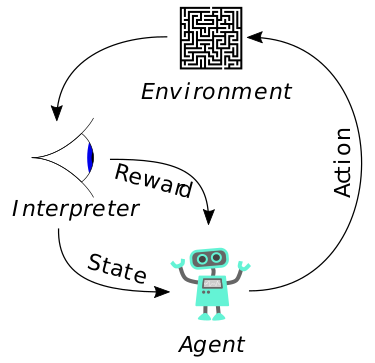
\includegraphics[width=60mm]{afbeeldingen/Reinforcement_learning_diagram.PNG}
			\caption[Routine bij Reinforcement Learning.]{Routine bij Reinforcement Learning.\cite{bron:reinforcementlearning}}
			\label{fig:reinforcemntLearning}
		\end{figure}
		
		Een van de vele mogelijke toepassingen van Reinforcement Learning is het aanleren van schaken door enkel mee te geven of het algoritme gewonnen of verloren heeft.



	\subsection{Leeralgoritmes en -technieken}
	Om \gls{ml} technieken toe te passen moet men gebruik maken van een bepaald wiskundig model dat is getraind op trainingsdata en hierdoor nieuwe data kan verwerken om voorspellingen te maken. Er bestaat een hele waaier aan mogelijke modellen. In de volgende paragrafen worden een aantal opties besproken waarna er de verschillende modellen met elkaar vergeleken worden.
	
		\subsubsection{Artifici\"ele Neurale Netwerken}
		\gls{ann} zijn een term dat gebruikt wordt om algoritmes te omschrijven die in staat zijn om een bepaalde taak te leren, en zichzelf te verbeteren. In de meeste gevallen worden er amper richtlijnen of een omschrijving meegegeven. Het systeem ontdekt zelf hoe deze regels in elkaar zitten\cite{carbonell1983overview}. Hierbij blijft de interpretatie van de input en de output wel nog belangrijk. Een bekend voorbeeld is het herkennen van de cijfers 0 tot 9. Hier wordt er niet aan het systeem verteld hoe de vorm van een getal er uit ziet. Het algoritme zal dit gaandeweg ontdekken, met behulp van vele voorbeelden waar het gebruik van kan maken. Met behulp van veel data kan een algoritme zichzelf verfijnen en zo nauwkeuriger bepaalde cijfers herkennen.
		
			\paragraph{Structuur van Neurale Netwerken}
			Een \gls{ann} is een verzameling van nodes die met elkaar verbonden zijn zoals neuronen in de hersens van een mens. Hierbij kan elke neuron een signaal doorgeven naar het volgende neuron waar het signaal verwerkt kan worden en weer doorgegeven kan worden. Hetzelfde principe geldt ook bij \gls{nn} met het verschil dat er meerdere lagen van nodes te onderscheiden zijn. 
	
		\begin{figure}
			\centering
			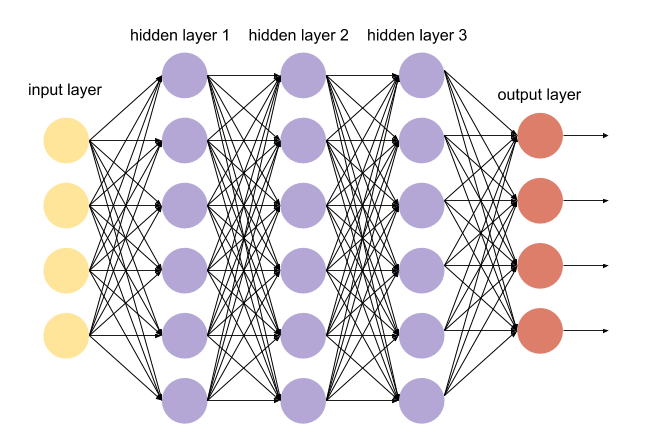
\includegraphics[width=140mm]{afbeeldingen/neuralNetwork3.PNG}
			\caption[Structuur van een Neuraal Netwerk.]{Structuur van een Neuraal Netwerk\cite{bron:machinelearningnetwork3}.}
			\label{fig:neuralNetworkStructuur}
		\end{figure}
		
			\subparagraph{Lagen}
			Er zijn drie soorten lagen te onderscheiden: een Input Layer, Hidden Layers en een Output Layer. Elke laag is verbonden met de volgende laag door middel van connecties tussen de verschillende nodes. In figuur ~\ref{fig:neuralNetworkStructuur} is de algemene vorm van een \gls{nn} te vinden.
		
				\begin{itemize}
					\item \textbf{Input Layer:} De eerste laag van elke \gls{nn} is de Input Layer. Deze bestaat uit een aantal inputnodes. Elke inputnode krijgt de ruwe data binnen waar er een operatie op uitgevoerd wordt en vervolgens bepaalde parameters doorgeeft aan de volgende laag. De wijze waarop data ge\"interpreteerd worden, vormt een belangrijk vertrekpunt voor het \gls{nn}.
					\item \textbf{Hidden Layers:}  Na de inputlaag komen een aantal Hidden Layers. Het aantal Hidden Layers en de hoeveelheid nodes binnen \'e\'en Hidden Layer kan vari\"eren van applicatie tot applicatie en is sterk gerelateerd aan de complexiteit van de toepassing.
					\item \textbf{Output Layer:} Na de Hidden Layers is de laatste laag de Output Layer. Hier worden de laatste operaties uitgevoerd en worden de eindwaarden verkregen waar het resultaat uit afgeleid kan worden.
				\end{itemize}
			
			\subparagraph{Nodes}
			 Lagen zijn opgebouwd uit meerdere nodes. Elke node krijgt een bepaald aantal inputs, verwerkt deze en geeft een bepaald aantal outputs. Deze inputs en outputs worden van node naar node doorgegeven via verbindingen. Elke node heeft met elke node in de volgende laag een connectie. Elke verbinding draagt een bepaald gewicht. Via dit gewicht kan men de invloed van de huidige node versterken of verzwakken in de volgende node.
	
			\subparagraph{Activatie functie}
			De mathematische functie die een node gebruikt voor het verwerken van inputs naar outputs heet de activatie functie. In figuur~\ref{fig:artificial_neuron} wordt de algemene vorm van een neuron besproken. Deze neuron heeft $m+1$ inputs $\left(  x_0 ~t.e.m.~  x_m\right) $ en bijhorende gewichten $\left(  w_0~  t.e.m. ~ w_m \right) $.
			Gebruikelijk wordt $x_0 = +1$ genomen. Hierdoor blijven er maar $m$ echte inputs over waardoor er voor een bepaalde output de functie \ref{eq:outputnode} opgesteld kan worden. Hierbij is $\phi$ een van de mogelijke transferfuncties die verder besproken zal worden.

			\begin{equation}
				y = \phi \left( \sum_{j=0}^{m}w_{j}x_j\right) 
				\label{eq:outputnode}
			\end{equation}
			
			\begin{figure}
				\centering
				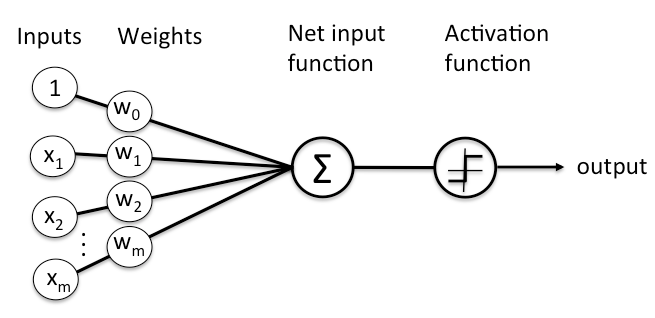
\includegraphics[width=80mm]{afbeeldingen/Artificial_neuron2.PNG}
				\caption[Algemene structuur van een node.]{Algemene structuur van een node\cite{bron:nnnode2}.}
				\label{fig:artificial_neuron}
			\end{figure}
			
			\subparagraph{Types activatiefuncties}
			De transfer functie of activatiefunctie is een belangrijk onderdeel van een laag in een \gls{ann}. De activatiefunctie transformeert inputs uit een vorige laag en transformeert deze naar een output. Deze output zal voor een volgende laag weer als input gebruikt worden. Door gebruik te maken van de juiste activatiefuncties kunnen er niet-lineaire eigenschappen aan het netwerk toegevoegd worden. Hieronder zullen enkele transferfuncties besproken worden.
			
			\begin{itemize}
				\item \textbf{Lineare Combinaties:} In dit geval is de output niets minder dan de gewogen som vermenigvuldigd met een constante waarbij zoals in formule~\ref{eq:gewogensomu} waar er nog een tweede constante wordt opgeteld.
				\item \textbf{Stapfunctie:} Hier wordt er gekeken naar de verkregen waarde van de gewogen som $u$ van $m+1$ inputs. Bedraagt deze waarde minder dan een bepaalde drempel $\theta$, dan wordt de output gelijkgesteld aan nul, bij een hogere waarde dan weer aan 1. Dit is te zien in formule ~\ref{eq:stapfunctie}. Dit type wordt vooral gebruikt om binaire inputs te verzorgen bij de volgende laag. 
			
				\begin{equation}\label{eq:gewogensomu}
					u =  \sum_{j=0}^{m}w_{kj}x_j
				\end{equation}
				
				\begin{equation}\label{eq:stapfunctie}
					y={\begin{cases}1&{\text{als }}u\geq \theta
					\\0&{\text{als }}u<\theta \end{cases}}
				\end{equation}
				
				\begin{equation}\label{eq:sigmoidfunctie}
					y={\frac {1}{1+e^{-u}}}
				\end{equation}
				
				\item \textbf{Sigmoid:} De Sigmoid functie\cite{han1995influence} is een mathematische functie zoals te zien is in figuur~\ref{eq:sigmoidfunctie}. Het heeft de karakteristieke 'S'-vorm zoals te zien is in figuur~\ref{fig:sigmoid}. Door deze activatiefunctie worden inputs omgezet in een waarde tussen 0 en 1 (of -1 en 1, afhankelijk van de conventie).
				\item \textbf{Rectifier:} De rectifier als activatiefunctie\cite{nair2010rectified} is een functie die enkel het positieve deel van zijn argument doorlaat. In vergelijking ~\ref{eq:rectifier} vind je de functie weer waar x de input is van de neuron. Deze is een vector aan waarden die zowel positief als negatief kunnen zijn. Deze functie is ook gekend onder de naam \textit{\gls{relu}}.
			
				\begin{equation}\label{eq:rectifier}
					f(x) = x^+ = max(0,x)
				\end{equation}
		
			\end{itemize}
			
			 
			
			\begin{figure}
				\centering
				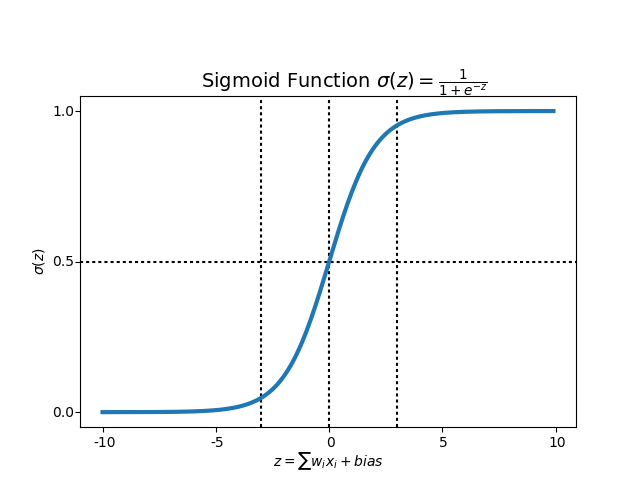
\includegraphics[width=100mm]{afbeeldingen/sigmoid2.PNG}
				\caption[De Sigmoid activatiefunctie.]{De Sigmoid activatiefunctie\cite{bron:sigmoidfoto}.}
				\label{fig:sigmoid}
			\end{figure}

	\subsubsection{Beslissingsboom} 
	Het gebruik van een beslissingsboom is een leermethode die met regelmaat terugkomt in de statistiek als een voorspellend model. Men maakt gebruik van observaties rond een bepaalde uitspraak. Men kwantificeert deze observaties zodat deze leiden naar een variabele outputwaarde. Indien deze waarde valt onder te verdelen in discrete klassen spreekt men over een \textit{classificatie boom}. Neemt de gezochte variabele eerder een continue vorm aan, dan maakt men gebruik van \textit{regressie bomen}.
	

	
		\paragraph{Structuur van een beslissingsboom}			
		Net zoals bij de \gls{nn} bestaat een beslissingsboom uit ver\hyp{}schillende lagen en nodes. Zoals te zien is in figuur ~\ref{fig:beslissingsBoom} wordt er in elke laag een onderscheid gemaakt op basis van een statement of parameter. Deze parameter kan een enkele inputwaarde zijn of een lineaire combinatie van meerdere inputwaarden. 
		
		Bij de nodes kan er onderscheid gemaakt worden tussen een gewone node en een eindnode. Bij elke gewone node wordt een bepaald statement geverifieerd en wordt er naar een node overgegaan in de volgende laag op basis van dit statement. Bij een eindnode is het niet meer mogelijk om door te gaan naar een volgende laag, maar wordt er een outputwaarde gegeven.
		
		\begin{figure}
			\centering
			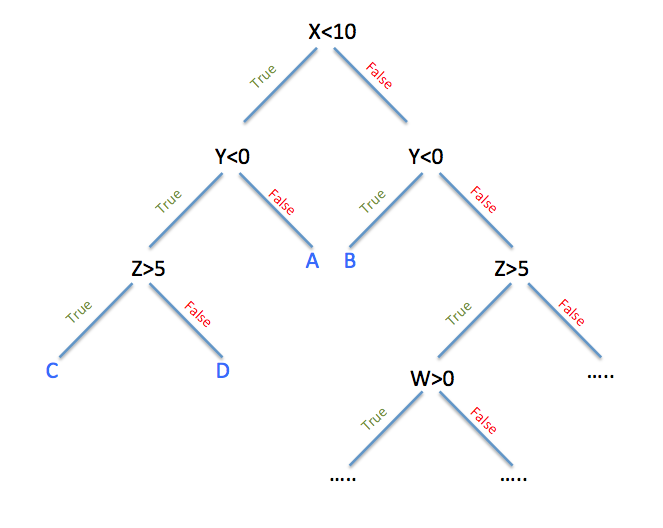
\includegraphics[width=80mm]{afbeeldingen/beslissingsBoom.PNG}
			\caption[Algemene structuur van een beslissingsboom.]{Algemene structuur van een beslissingsboom\cite{bron:beslissingsboom}.}
			\label{fig:beslissingsBoom}
			%bron: https://medium.com/machine-learning-bites/machine-learning-decision-tree-classifier-9eb67cad263e
		\end{figure}
		
		
	
	
	\subsubsection{Support Vector Machines}
	\gls{svm} of ook wel gekend als support vector networks is een model dat veelvuldig gebruikt wordt in classificatie en regressie-analyse. Een belangrijke toepassing van \gls{svm} is het verdelen van objecten in twee verschillende klassen op basis van een aantal kenmerken. Het is dus onder meer een binaire classificeerder. Om aan de hand van kenmerken een onderverdeling te maken moeten deze kenmerken eerst omgezet worden in een vectorruimte. In de trainingsfase wordt er getracht een zo optimaal mogelijke scheiding tussen beide klassen te vinden. Deze optimale scheiding wordt ook wel een \textit{hypervlak} genoemd en ligt op een zo groot mogelijke afstand tussen de dichtstbijgelegen objecten van beide klasses of support vectors. in figuur ~\ref{fig:supportVectorMachines} kan u een tweedimensionaal voorbeeld vinden. Hierin is scheidingslijn H1 geen acceptabele scheiding omdat er objecten van de zwarte klasse fout geclassificeerd worden. H2 is acceptabel maar is nog niet optimaal aangezien er weinig foutmarge is voor een nieuw object. H3 is het hypervlak omdat de foutenmarge tussen de twee klassen zo groot mogelijk is. Deze methode is niet alleen bruikbaar in toepassingen met een lineaire scheiding. Ook in niet-lineaire gevallen kan men een transformatie uitvoeren om toch een lineaire scheiding te bekomen. Deze hervorming wordt ook wel de \textit{kernel trick}\cite{sun2018kernel} genoemd. 
	
	
	\begin{figure}
		\centering
		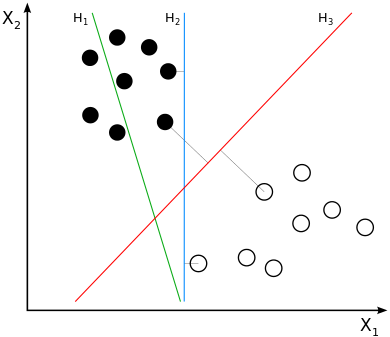
\includegraphics[width=80mm]{afbeeldingen/supportVectorMachines.PNG}
		\caption[Tweedimensionale Support Vector Machine.]{Tweedimensionale Support Vector Machine\cite{bron:supportvectormachines}.}
		\label{fig:supportVectorMachines}
		%bron: https://subscription.packtpub.com/book/big_data_and_business_intelligence/9781788994170/5/ch05lvl1sec36/support-vector-machines
	\end{figure}
		
			
	\subsubsection{Regressie Analyse}
	Regressie Analyse is een techniek uit de statistiek\cite{sieben2009logistische}, die gebruikt wordt om gegevens te analyseren met een specifiek verband. Er bestaat vaak een relatie tussen een afhankelijke variabele en \'e\'en (of meerdere) onafhankelijke variabelen. De meest voorkomende vorm van regressie analyse is de lineaire regressie, waar men op zoek gaat naar de functie die het dichtst aanleunt bij de data. De functie moet wel vervullen aan specifieke criteria, zo moet de functie bijvoorbeeld een bepaalde orde hebben. Regressie analyse wordt vooral gebruikt voor het voorspellen van nieuwe data of gebeurtenissen. In figuur ~\ref{fig:regressieAnalyse} kan je een voorbeeld van lineaire regressie vinden.

	\begin{figure}
		\centering
		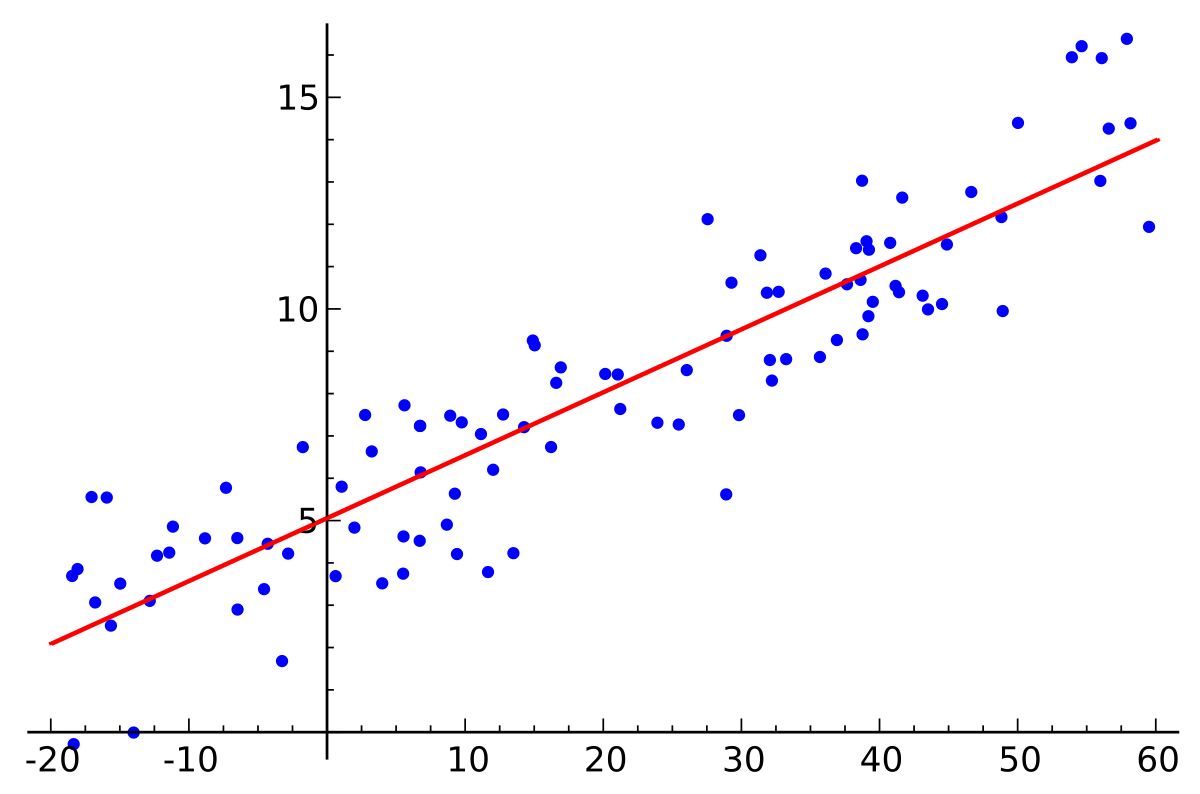
\includegraphics[width=80mm]{afbeeldingen/regressieAnalyse.PNG}
		\caption[Voorbeeld van Lineaire Regressie.]{Voorbeeld van Lineaire Regressie\cite{bron:regressieanalyse}.}
		\label{fig:regressieAnalyse}
		
		%bron: https://en.wikipedia.org/wiki/Regression_analysis
	\end{figure}
	
	\subsubsection{Bayesian Netwerken}
	Bayesian Netwerken, ook wel probabilistische netwerken genoemd, zijn structuren waarin data op probabilistische wijze geanalyseerd kunnen worden. Dit wil zeggen dat men als output niet enkel de outputs maar ook de onzekerheid hierop krijgt. Men maakt gebruik van gerichte grafen. Hierin bestaan de knopen uit variabelen en de arcs beschrijven de conditionele afhankelijkheden tussen de verschillende knopen. Bayesian Netwerken worden vooral gebruikt om te analyseren wat de bepalende oorzaak is voor een zekere gebeurtenis. 
	
	\subsubsection{Genetische Algoritmes}
	Genetische Algoritmes zijn een heuristiek ge\"inspireerd op het principe van natuurlijke selectie en zijn een klasse binnen evolutionaire algoritmes. Dit type algoritme kan gebruikt worden om oplossingen te vinden in optimalisatie- en zoekproblemen. Door te steunen op biologische principes zoals mutatie, selectie en kruisbestuiving worden er nieuwe \textit{chromosomen} gegenereerd die mogelijks een betere oplossing geven voor een bepaald probleem.
	
\subsection{Keuze voor een Machine Learning-methode }	
% https://elitedatascience.com/machine-learning-algorithms

Om de keuze voor een bepaalde \gls{ml}-techniek te verantwoorden, zal dit hoofdstuk de voor- en nadelen behandelen van de voornaamste technieken die via regressie of classificatie toegepast kunnen worden\cite{bron:mlalgoritmes}.

	\subsubsection{Regressie}

	\begin{itemize}
		\item \textbf{Neurale Netwerken:}
			\subitem Voordelen: Neurale netwerken zijn de meest gebruikte toepassing in verschillende domeinen. \gls{nn} kunnen uitstekend omgaan met onder meer beeld-, audio- en tekstdata en deze verwerken. Verder kan de architectuur ook nog gemakkelijk aangepast worden aan de toepassing door te vari\"eren in het aantal lagen of nodes. Het gebruik van de hidden layers vermindert ook het hanteren van feature engineering. 
			
			\subitem Nadelen: Neurale netwerken zijn minder bruikbaar voor \textit{general-purpose} algoritmes door de grote hoeveelheid data die er voor nodig zijn. In dat geval is het beter om voor beslissingsbomen te kiezen. Bovendien vragen ze veel computationeel vermogen voor het trainen van het netwerk en vragen veel expertise voor kleine aanpassingen zoals aan de architectuur of hyperparameters. 
			
		\item \textbf{Regression Trees:}
			\subitem Voordelen: Beslissingsbomen met nadruk op regressie zijn in staat om niet-lineaire relaties te leren en zijn robuust voor uitschieters in de te verwerken dataset.
			
			\subitem Nadelen: Regression trees zijn vatbaar voor overfitting indien er te veel gebruik gemaakt wordt van branches. Bij bomen is het ook mogelijk om vertakkingen te blijven maken tot het een exacte kopie voorstelt van de trainingsdata.
			
		\item \textbf{Lineaire Regressie:}
			\subitem Voordelen: Dit is een eenvoudige methode om zowel te begrijpen als uit te leggen. Daarnaast kan er een eenvoudige bescherming tegen overfitting ge\"implementeerd worden.
			
			\subitem Nadelen: Niet-lineaire relaties zijn een zwak punt voor lineaire regressie. Het is moeilijk om een correcte fitting te vinden voor een gegeven ingewikkelde relatie. Bovendien is het onvoldoende flexibel om complexe patronen op te vangen.

	\end{itemize}

	\subsubsection{Classificatie}
	
	\begin{itemize}
		\item \textbf{Neurale Netwerken:}
			\subitem Voordelen: \gls{nn} blijven uitstekend presteren bij het classificeren van audio-, tekst- en beeldherkenning.
			
			\subitem Nadelen: Er is nood aan grote hoeveelheden data om het model te trainen en minder geschikt als general-purpose algoritme.
			
		\item \textbf{Classification Trees:}
			\subitem Voordelen: Verrichten zeer goed werk in praktijk. Ze zijn robuust voor uitschieters, schaalbaar voor meerdere klassen en kunnen niet-lineaire grenzen op natuurlijke wijze modelleren dankzij de hi\"erarchische structuur.
			
			\subitem Nadelen: Classification trees zijn vatbaar voor overfitting indien er te veel gebruik gemaakt wordt van branches. Bomen hebben vaak de neiging om branches aan te maken tot het een exacte kopie voorstelt van de trainingsdata.
			
		\item \textbf{Support Vector Machines:}
			\subitem Voordelen: \gls{svm} zijn in staat om niet-lineaire beslissingsgrenzen te modelleren en hebben een sterke robuustheid tegen overfitting, vooral in hogere dimensionale vectorruimtes.
			
			\subitem Nadelen: \gls{svm} zijn heel erg geheugen intensief. Ze vragen ook meer expertise in het afstemmen door het grote aanbod in mogelijke kernels. \gls{svm} hebben de eigenschap om minder effectief te zijn bij het schalen naar grotere datasets. 
			
		\item \textbf{Geregulariseerde Regressie:}		
			\subitem Voordelen: Outputs hebben een  gemakkelijk leesbare probabilistische interpretatie. Ook kan er bescherming tegen overfitting ge\"implementeerd worden en kunnen modellen eenvoudig ge\"updatet worden.
			
			\subitem Nadelen: Niet-lineaire relaties zijn een zwak punt voor lineaire regressie. Het is moeilijk om een correcte fitting te vinden voor een gegeven ingewikkelde relatie. Bovendien is het onvoldoende flexibel om complexe patronen op te vangen.

			
	\end{itemize}

	\subsubsection{Besluit}
	Na een afweging gedaan te hebben van de voor- en nadelen van de voornaamste kandidaten bij zowel regressie als classificatie toepassingen zal in het kader van deze thesis voor \gls{nn} gekozen worden. Er wordt vooral gesteund op het feit dat \gls{nn} uitstekend werk levert in beide klassen in het analyseren van data. Bovendien zijn de voornaamste nadelen minder van toepassing in het kader waarin \gls{nn} toegepast zal worden. Het is vooral van belang hoe de netwerken in de executiefase presteren. Het trainen van de verschillende netwerken met grote hoeveelheden data kan op aparte systemen gebeuren. De trainingsfase is dus minder van belang voor het doel van deze thesis. Bovendien is het niet nodig om een breed general-purpose netwerk te voorzien.
	
	Een mogelijk alternatief voor \gls{nn} is het gebruiken van Regressie Analyse. De bepalende factor hiervoor is dat het karakter van de verscheidene applicaties vaak uit lineaire relaties bestaat. 
		
		
		
		
 
	

\newpage	

%------------------------------------------------------------------------------	
\section{Evolutie Single Board Computers}
Een \gls{sbc} is een volledige computer gemaakt op 1 enkele printplaat. Het bevat onderdelen zoals een microprocessor, geheugen, inputs en outputs. De eerste \gls{sbc} werd ontwikkeld als een voorstel-hulpmiddel bij educatieve doelstellingen of het gebruik als een embedded computer controller. Tegenwoordig zijn ook vele (draagbare) computers ge\"integreerd op \'e\'en printplaat. Het grote verschil met (draagbare) computers is dat er geen nood is aan expansion slots zoals bijvoorbeeld voor RAM-geheugen of een \gls{gpu}.
	\subsection{Geschiedenis}
	De eerste echte SBC was de zogenaamde "dyna-micro"\space uit figuur ~\ref{fig:eersteSBC} die later de naam "MMD-1" (Mini-Micro Designer 1) kreeg\cite{bron:fotoeerstesbc}. Dit toestel werd uitgegeven in 1976 en werd populair doordat het werd gepresenteerd in het destijds 'BugBook'. Een andere vroege \gls{sbc} was de KIM-1 (Keyboard Input Monitor 1) uit hetzelfde jaar. Beide machines werden voor ingenieurs geproduceerd en ontworpen maar vonden een breed publiek onder de hobbyisten waar het heel populair werd. Later kwamen nog andere namen zoals de Ferguson Big Board en de Nascom.

	\begin{figure}
		\centering
		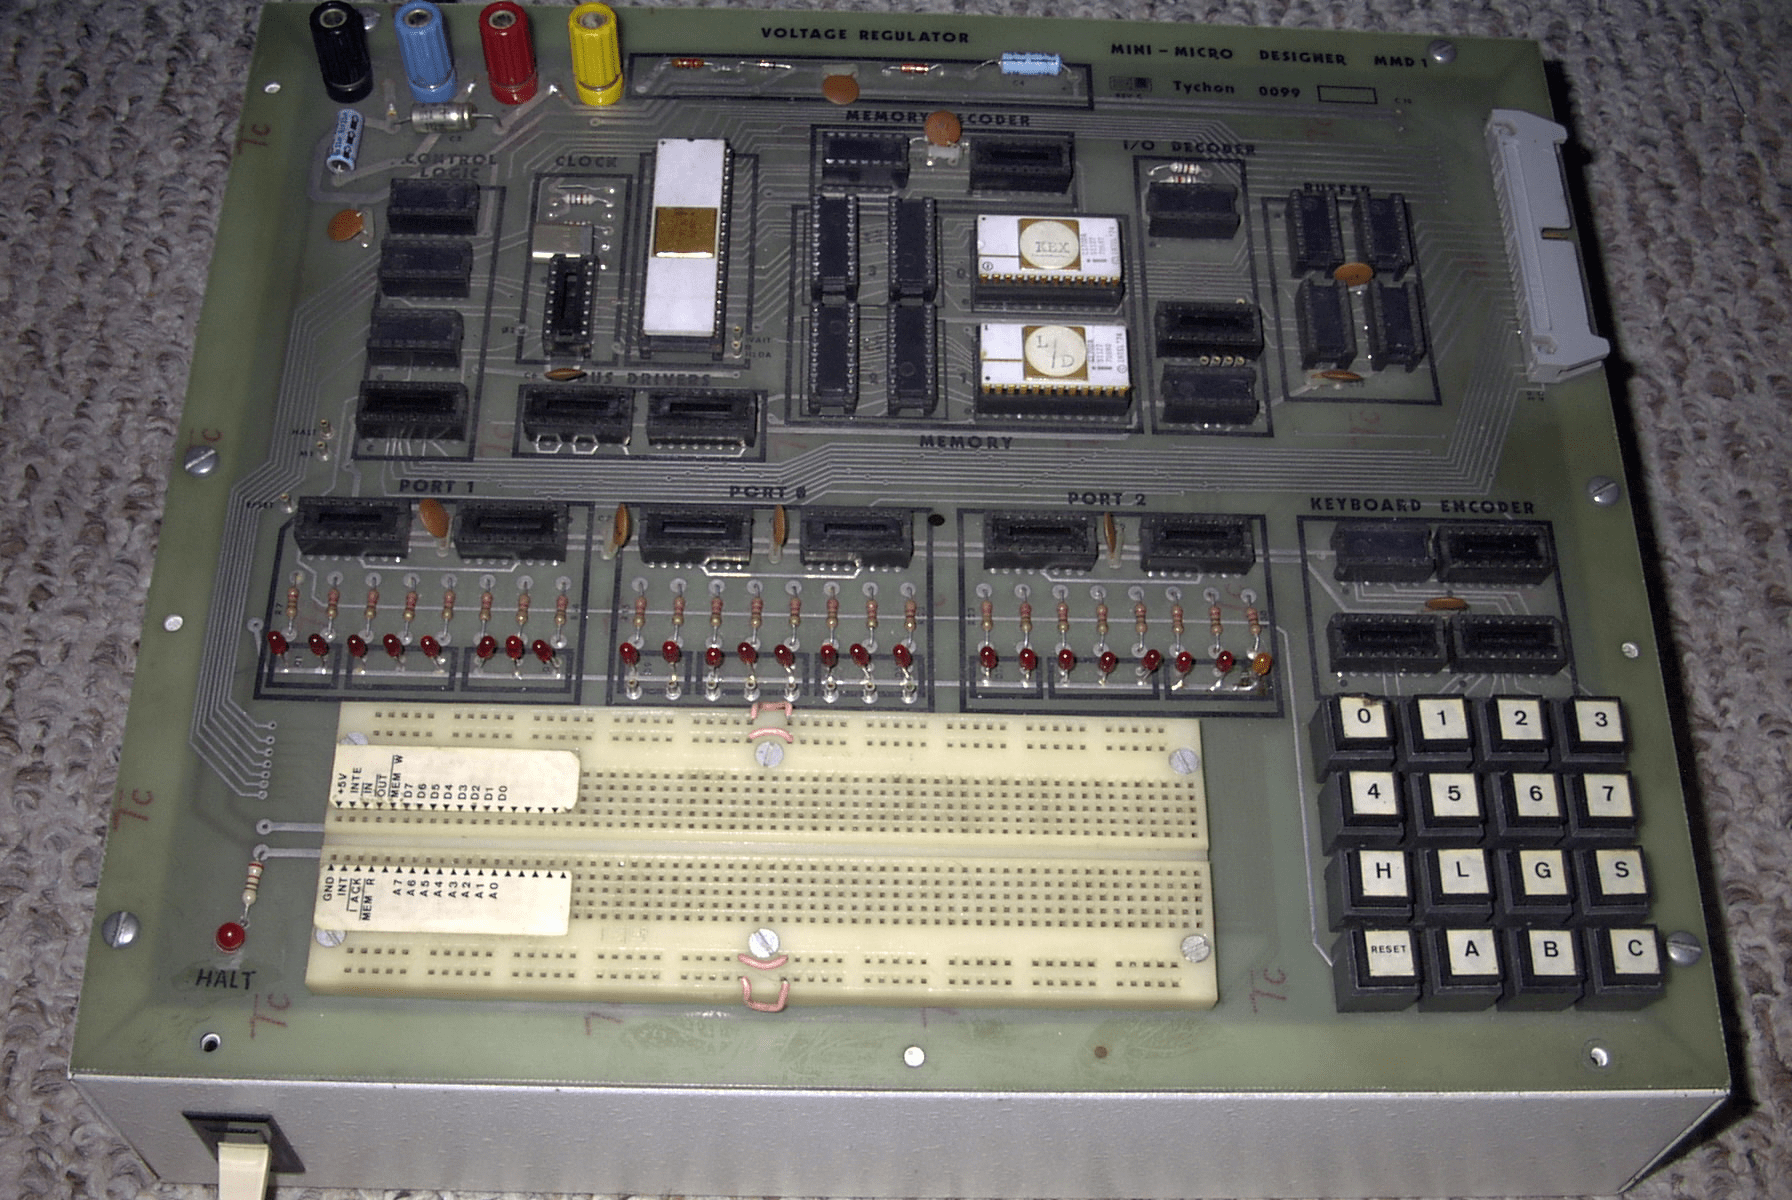
\includegraphics[width=120mm]{afbeeldingen/Early_1976_MMD1_Prototype_most_chips_removed.PNG}
		\caption[Eerste SBC: MMD-1.]{Eerste \gls{sbc}: MMD-1\cite{bron:fotoeerstesbc}.}
		\label{fig:eersteSBC}
	\end{figure}
	
	Naarmate de markt voor desktops en PC's groeide, nam de belangstelling voor \gls{sbc} in computers meer en meer af. De focus van de markt werd verlegd naar een moederbord met de belangrijkste componenten en dochterborden voor periferiecomponenten zoals seri\"ele poorten. De voornaamste reden hiervoor was dat de componenten groot waren. Alle onderdelen op dezelfde printplaat zou zorgen voor een onpraktisch ontwerp met grote afmetingen. Deze beweging was echter tijdelijk en naarmate de vorderende technologie kleinere componenten kon leveren, werden onderdelen terug naar het mainframe verschoven. Tegenwoordig kunnen de meeste moederborden terug als \gls{sbc} beschouwd worden. 

	
	In het jaar 2004 werd er in Itali\"e een nieuwe microcontroller uitgebracht onder de naam "Arduino". Dit ontwerp had, naast het voordeel van compact en goedkoop te zijn, ook nog eenvoudigheid mee. Door de eenvoud werd het Arduino-platform snel populair onder techneuten van alle soorten. 
	Twee jaar later bracht de Universiteit van Cambridge een nieuwe goedkope \gls{sbc} uit. De bekende Raspberry Pi werd gelanceerd voor de prijs van \$35. Het hoofddoel van dit project was een nieuw leermiddel om te programmeren maar werd door het grote aantal applicaties ook zeer populair. \label{raspberry}
	
	De laatste jaren kende een grote explosie aan nieuwe \gls{sbc}s. Een hele reeks nieuwe namen verschenen. Banana Pi, Beaglebone, Intel Galileo, Google Coral Dev en Asus Tinker Board zijn maar enkele van de vele voorbeelden. Deze toestellen hebben vaak een processor gebaseerd op de x86- of ARM-series en maken gebruik van een Linux besturingssysteem zoals Debian.
	

% https://nl.wikipedia.org/wiki/Singleboardcomputer

\newpage


%------------------------------------------------------------------------------
\section{Assortiment aan 'off the shelf' toestellen}
In deze sectie wordt er een kort overzicht gegeven van de te gebruiken \gls{sbc}s binnen deze thesis. Er werd gekozen om met vijf verschillende toestellen te werken die in de edge toegepast kunnen worden. Daarnaast wordt er er ook met een personal Computer gewerkt. De gebruikte devices verschillen in verscheidene aspecten. Zo zijn er zowel goedkope als kostelijkere apparaten, populaire boards als minder gekende \gls{sbc}s. Er zijn toestellen met hele geavanceerde processoren die specifiek voor \gls{ml} zijn ontworpen, maar ook processoren die ontwikkeld zijn voor meer algemenere toepassingen. De specificaties van de verscheidene toestellen worden ook meegegeven. In tabel \ref{tab:specdevices} kan er een samenvatting van de belangrijkste specificaties gevonden worden.

	\subsection{Beaglebone AI}
	\gls{bbai} is een \gls{sbc} dat verder bouwt op de succesvolle  BeagleBoard-series\citep{bron:bbai}. Het is een open source project met een op Linux gebaseerd aanpak. De \gls{bbai} probeert het gat tussen kleinere \gls{sbc} en krachtigere industri\"ele computers te overbruggen. Met behulp van de krachtige Texas Instruments AM5729 CPU kunnen ontwikkelaars de krachtige \gls{soc} gebruiken om een hele brede waaier aan toepassingen te verwezenlijken. De \gls{bbai} maakt het toegankelijker om het \gls{ai}-terrein te ontdekken en te verkennen. Door gebruik te maken van onder andere \gls{eve} cores die steunen op een geoptimaliseerde TIDL machine learning OpenCL API, kan je terecht in alledaagse automatisatie in industri\"ele, commerci\"ele en thuisapplicaties.
	
	
	\subsubsection{Specificaties}
	\begin{itemize}
		\item \textbf{GPU:} Niet van toepassing
		\item \textbf{CPU:} Texas Instruments AM5729
		\item \textbf{Memory:} 16 GB on-board eMMC flash
		\item \textbf{Storage:} 1GB RAM + micro SD-slot
		\item \textbf{Power:} 5 Watt
		\item \textbf{Prijs:} \$139.37
	\end{itemize}
	
	% https://beagleboard.org/ai

	\newpage

	\subsection{Coral Dev Board}
	De Coral Dev Board is een development board gemaakt door het Amerikaanse technologiebedrijf Google\citep{bron:coraldev}. Het board is ontworpen om het ontwikkelen van on-device ML producten te vergemakkelijken. Hiervoor heeft het een aantal belangrijke voordelen gekregen door zijn designers. Het is vooral de aangepaste \gls{tpu} \gls{ai} chip die hier opvalt. De \gls{tpu} is een \gls{asic} speciaal ontworpen voor \gls{nn} \gls{ml}, en is in staat om video in hoge resolutie te analyseren aan 30 frames per second. Deze \gls{som} is geoptimaliseerd om Tensorflow Lite te kunnen draaien aan meerdere \gls{tops}.
	
		\subsubsection{Specificaties}
		\begin{itemize}
			\item \textbf{GPU:} Integrated GC7000 Lite Graphics
			\item \textbf{CPU:} NXP i.MX 8M SOC (quad Cortex-A53, Cortex-M4F) + coprocessor Google Edge TPU
			\item \textbf{Memory:} 8 GB on-board eMMC flash
			\item \textbf{Storage:} 1GB RAM LPDDR4 + micro SD-slot
			\item \textbf{Power:} 0.5 watts for each TOPS - 2 Watt
			\item \textbf{Prijs:} \$149.99
		\end{itemize}
	
	% https://venturebeat.com/2019/10/22/googles-coral-ai-edge-hardware-launches-out-of-beta/
	
	\subsection{Nvidia Jetson Nano}
	De Jetson Nano is een populair bord uit de Jetson Series van Nvidia\citep{bron:jetsonnano}. Het is een kleine maar krachtige computer ontwikkeld voor embedded applicaties en low-power \gls{ai}-\gls{iot}. Deze \gls{sbc} wordt ondersteund door meerdere bibliotheken in sectoren zoals deep learning, computer vision, beeld en multimedia. De hardware bevat zowel een \gls{gpu} als een \gls{cpu}. De \gls{gpu} bestaat uit een krachtige Maxwell architectuur die beeld kan decoderen aan 500 MP/sec. De \gls{cpu} is van het type Cortex-A57 met 4 kernen.
	
		\subsubsection{Specificaties}
		\begin{itemize}
			\item \textbf{GPU:} 128-core Maxwell met 128 CUDA-cores
			\item \textbf{CPU:} Quad-core ARM A57 @ 1.43 GHz
			\item \textbf{Memory:} 4 GB 64-bit LPDDR4 25.6 GB/s
			\item \textbf{Storage:}  micro SD-slot
			\item \textbf{Power:} 5 - 10 W
			\item \textbf{Prijs:} \$99
		\end{itemize}	
	
	% https://developer.nvidia.com/embedded/jetson-nano

	\newpage
	
	\subsection{Nvidia Jetson TX2}
De TX2, uit de zelfde Jetsonserie, is de high end versie van de hiervoor besproken Nano\citep{bron:jetsontx2}. Het is het snelste en meest power-effici\"entst van de embedded \gls{ai} toestellen die gebruikt zal worden in deze thesis. De TX2 verbruikt een 7.5 Watt en brengt het zware \gls{ai}-rekenwerk naar de edge. Zijn bekwame \gls{gpu} met 256 CUDA kernen en een duo \gls{cpu} zijn in staat om de meest geavanceerde Machine Leertechnieken uit te voeren. De grote geheugenvoorzieningen zorgen bovendien dat de datasetgrootte geen beperkende factor meer kan spelen. Verder wordt er nog gezorgd voor een grote ondersteuning via een grote variatie aan hardware interfaces. Hierdoor wordt het integreren van producten aanzienlijk makkelijker.

\subsubsection{Specificaties}
\begin{itemize}
	\item \textbf{GPU:} 256-core NVIDIA Pascal GPU architecture with 256 NVIDIA CUDA cores
	\item \textbf{CPU:} Dual-Core NVIDIA Denver 2 64-Bit \& CPU Quad-Core ARM Cortex-A57 MPCore
	\item \textbf{Memory:} 8GB 128-bit LPDDR4 Memory 1866 MHx - 59.7 GB/s
	\item \textbf{Storage:}  32GB eMMC 5.1
	\item \textbf{Power:} 7,5 - 15 W
	\item \textbf{Prijs:} \$399
\end{itemize}	

% https://developer.nvidia.com/embedded/jetson-tx2


	\subsection{Raspberry Pi}
	De laatste \gls{sbc} die hier besproken wordt, is de Raspberry Pi 4\citep{bron:rpi4}. Dit is een heel goedkoop en eenvoudig device. Het komt uit de heel gekende Raspberry-reeks zoals al besproken in paragraaf \ref{raspberry}. In deze thesis wordt gebruik gemaakt van het model 3 B. De specificaties kunnen hieronder gevonden worden. Het heeft een behoorlijke Cortex Quad core-\gls{cpu} met degelijk geheugen die uitgebreid wordt door een SD-kaart. 
	
		\subsubsection{Specificaties}
		\begin{itemize}
			\item \textbf{CPU:} Broadcom BCM2711, Quad core Cortex-A72 (ARM v8) 64-bit SoC @ 1.5GHz
			\item \textbf{Memory:} 1GB, 2GB or 4GB LPDDR4-3200 SDRAM
			\item \textbf{Storage:}  micro SD-kaart
			\item \textbf{Power:} 2,8 - 5,2 W
			\item \textbf{Prijs:} \$35
		\end{itemize}	
	
	% https://www.raspberrypi.org/products/raspberry-pi-4-model-b/
	
	
	\newpage
		
	\subsection{Personal Computer: Lenovo Legion Y520}
	De gebruikte personal computer is van het technologiemerk Lenovo. De Legion-serie biedt een breed gamma gamingcomputers aan het publiek. Het gebruikte Y520-model\cite{bron:lenovolegion} is samengesteld uit een aantal krachtige onderdelen. Zo bevat het model een sterke \gls{gpu}, de NVIDIA  GTX 1050, en \gls{cpu}, de Intel Core i5-7300HQ, zorgen in combinatie met een hoge kloksnelheid voor een hoge performantie. De kloksnelheid bedraagt in idle-toestand 2500 MHz en onder load kan dit door gebruik te maken van \textit{dynamic frequency changing} opgedreven worden tot 3300 MHz. De grote hoeveelheden RAM-geheugen en opslagruimte staan toe om meer eisende programma's te runnen op het toestel. Deze grote performantie vraagt wel meer vermogen en een hogere prijs dan de tot nu toe vermelde toestellen. Bij het vermelde vermogen zitten randapparatuur zoals scherm en toetsenbord ook in verwerkt.
	
	
	\subsubsection{Specificaties}
	\begin{itemize}
		\item \textbf{GPU:} NVIDIA GeForce GTX 1050 Ti Mobile
		\item \textbf{CPU:} Intel Core i5-7300HQ
		\item \textbf{Memory:} 8GB DDR4-2400
		\item \textbf{Storage:}  128 GB SSD, 1 TB HDD
		\item \textbf{Power:} 10 - 100 W
		\item \textbf{Prijs:} \$981
	\end{itemize}	
	
	% https://www.notebookcheck.net/Lenovo-Legion-Y520-15IKBN-7300HQ-GTX-1050-Ti-FHD-Laptop-Review.256682.0.html
	
	
	\begin{table}[]
		\centering
	\begin{tabular}{ccccc}
	\hline
	Toestel                              & GPU                  & CPU                    & Power {[}W{]} & Price {[}\${]} \\ \hline
	\multicolumn{1}{c|}{Beaglebone Ai}   & n.v.t.               & TI AM5729              & 5             & 139,37         \\
	\multicolumn{1}{c|}{Coral Dev Board} & GC7000 Lite Graphics & NXP i.MX 8M + Edge TPU & 2             & 149,99         \\
	\multicolumn{1}{c|}{Jetson Nano}     & 128-core Maxwell     & Quad-core ARM A57      & 5 -10         & 99             \\
	\multicolumn{1}{c|}{Jetson TX2}      & 256-core Pascal      & Denver 2 \& Cortex-A57 & 7,5-15        & 399            \\
	\multicolumn{1}{c|}{Raspberri pi}    & n.v.t.               & BCM2711, Cortex-A72    & 2,8 - 5,2 W   & 35             \\
	\multicolumn{1}{c|}{PC}              & GeForce GTX 1050 Ti  & Intel Core i5-7300HQ   & 10 - 100 W    & 981            \\ \hline
	\end{tabular}
		\caption{Specificaties van gebruikte toestellen.}
		\label{tab:specdevices}
	\end{table}
\newpage

%------------------------------------------------------------------------------
\section{Benchmarking van Machine Learning algoritmes}
\label{benchmark}

Om betekenisvolle resultaten te verkrijgen is het nodig om een goed bruikbare en representatieve benchmark op te stellen. Een benchmark is een onderzoek waarbij de prestaties van programma's met elkaar vergeleken worden. Dit komt tot stand als elk programma op identieke wijze wordt onderzocht. Door de prestaties van programma's met elkaar te vergelijken is het mogelijk de performantie van de verscheidene \gls{sbc} in kaart te brengen. Hoe de benchmark exact in elkaar zit is gebonden aan de kwaliteitscriteria die onderzocht worden. Om ervoor te zorgen dat de benchmark onafhankelijk is van zowel het specifiek veld als toepassing, is het nodig dat er aan een aantal karakteristieken wordt voldaan\cite{libuttibenchmarking}.

\begin{itemize}
	\item \textbf{Vergelijkbaarheid:} Benchmarks moeten zodanig opgesteld zijn, dat het evident is wat ze vergelijken en de conclusie ondubbelzinnig is.
	\item \textbf{Herhaalbaarheid:} Bij het herhalen van de test onder gelijkaardige omstandigheden moeten gelijkaardige resultaten gehaald worden.
	\item \textbf{Goed gedefinieerde methodologie:} De werkwijze, methode en aannames moeten voldoende gedocumenteerd en gestaafd worden.
	\item \textbf{Configureerbaar:} Benchmarks moeten beschikken over parameters die aangepast kunnen worden naar het specifieke probleem dat wordt behandeld.
\end{itemize}


	\subsection{Bestaande benchmarks}
	De ontwikkelaars van de Jetson Nano vermelden op de Nvidia-website\cite{bron:nanobenchmark} verschillende \gls{dlib} waarbij de auteur verscheidene op voorhand getrainde \gls{dl} modellen toepassen op het Nano bord. Deze modellen zijn gebaseerd op een brede waaier aan populaire \gls{ml} frameworks zoals Tensorflow, Caffe, PyTorch en Keras. Bovendien zijn de applicaties ook gespreid over meerdere toepassingen zoals beeldherkenning, objectdetectie, positiebepaling en anderen. %De modellen en resultaten zijn te vinden in figuur \ref{fig:nanobenchmark}.

%	\begin{figure}
%		\centering
%		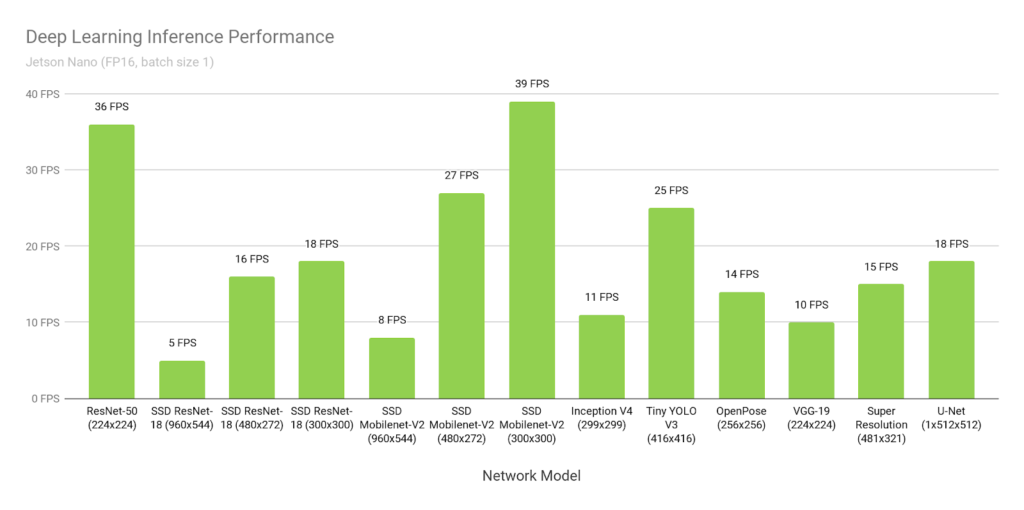
\includegraphics{afbeeldingen/NanoBenchmark.png}
%		\caption{Modellen en resultaten van de benchmark op de Jetson Nano. \\Afbeelding te vinden op https://devblogs.nvidia.com/jetson-nano-ai-computing/.\\ Website werd geraadpleegd op 17/02/2020.}
%		\label{fig:nanobenchmark}
%	\end{figure}

	Ook voor de Jetson TX2 bestaat er een benchmark zoals voorgesteld in \cite{bordignonbenchmarking}. Het gaat over een general-purpose benchmark die een aantal parameters controleert. Het gaat over variabelen zoals \gls{fps}, \textit{inference time}, \gls{gpu} temperatuur en geheugen verbruik. Met inference time wordt de tijd bedoeld om een berekening te doen in \gls{gpu} en \gls{cpu} m.a.w. de latency veroorzaakt door de \gls{sbc}. Deze gegevens worden uit de data gehaald door middel van verschillende \gls{dl} modellen toe te passen op \gls{cnn}. Deze modellen passen ze toe op twee verschillende datasets: Microsoft COCO dataset voor objectdetectie, een foto bank met een grote verscheidenheid aan categorie\"en, en de KITTI Stereo Vision databank. De KITTI-databank bestaat uit 400 foto's specifiek bedoeld als benchmark fotoset.
	
	Er bestaan ook meer algemenere benchmarks om vergelijkingen tussen computersystemen te maken. Zo bestaat er ook de LINPACK benchmarks\cite{bron:LINPACKBENCHMARK}. Dit is een programma waar de snelheid gemeten kan worden waarmee een computer in staat is om een $n~ $bij$~ n$ matrix van lineaire vergelijkingen op te lossen. Ondanks dat het een veelgebruikte benchmark is, zijn er wel nog bedenkingen over de werkwijze. Zo bestaat de kerntaak maar uit een enkele computationele taak die onmogelijk de algemene performantie van een systeem kan weergeven. Desondanks geeft de LINPACK benchmark een goed karakteristiek beeld van computersystemen. De meest bekende toepassing waar LINPACK in toegepast wordt is de ranking van de beste 500 supercomputers ter wereld\cite{bron:LINPACKBENCHMARK500}

% ==============================================> Benchmark instructies https://devtalk.nvidia.com/default/topic/1050377/jetson-nano/deep-learning-inference-benchmarking-instructions/

% http://www.cs.toronto.edu/~serailhydra/publications/tbd-iiswc18.pdf



	

% waarom op de edge plaatsen van EBC (Voor en Nadelen) (miss meer situring)
% Specs van de verschillende boards 